\section{Брокеры сообщений}
\subsection{RabbitMQ}

RabbitMQ — это программное обеспечение для организации очередей сообщений; его также называют брокером сообщений или менеджером очередей. Проще говоря, это система, в которой определяются очереди, к которым подключаются приложения, чтобы передать одно или несколько сообщений.

Сообщение может содержать любую информацию. Например, в нём могут передаваться данные о процессе или задаче, которую нужно запустить в другом приложении (возможно, находящемся на другом сервере), либо это может быть просто текстовое сообщение. Брокер хранит сообщения, пока приложение-получатель не подключится и не заберёт их из очереди. Затем получатель обрабатывает сообщение.

Брокер сообщений действует как посредник между различными сервисами (например, веб-приложением). Он позволяет снизить нагрузку и сократить время отклика веб-серверов, передавая ресурсоёмкие или длительные операции стороннему компоненту, у которого нет других задач.

Очереди сообщений позволяют веб-серверам быстро отвечать на запросы, не выполняя сразу тяжёлые вычисления, которые могли бы задержать ответ. Кроме того, очереди удобны, когда нужно доставить одно сообщение нескольким потребителям или сбалансировать нагрузку между рабочими процессами.

Потребитель забирает сообщение из очереди и начинает его обрабатывать, в то время как производитель продолжает ставить новые сообщения в очередь. Потребитель может находиться на совершенно другом сервере, чем производитель, или на том же самом. Запрос может быть сформирован на одном языке программирования, а обработан — на другом. Главное, что оба приложения взаимодействуют только через передаваемые сообщения, что обеспечивает их слабую связанность.

\begin{figure}[h!]
    \centering
    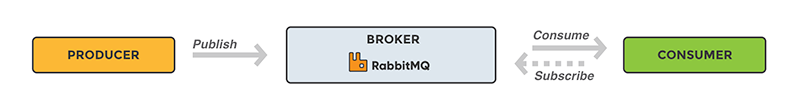
\includegraphics[width=0.7\textwidth]{styles/diploma/inc/rabbitmq1.png} 
    \caption{Общее представление работы RabbitMQ}
    \label{fig:example}
\end{figure}

Сообщения публикуются не напрямую в очередь: сначала продюсер отправляет их на exchange (обменник). Именно обменник отвечает за маршрутизацию сообщений в разные очереди с помощью биндингов и ключей маршрутизации (routing keys). Биндинг представляет собой связь между очередью и обменником.

Порядо отправки сообщения в RabbitMQ:
\begin{enumerate}[label=., leftmargin=3em]
\item Продюсер публикует сообщение в обменник. При создании обменника  обязательно указывается его тип (об этом — позже).
\item Обменник получает сообщение и решает, как его направить. При этом он учитывает тип обменника и свойства сообщения, например routing key.
\item К обменнику создаются биндинги, связывающие его с очередями. На рисунке показано два биндинга к двум различным очередям. В зависимости от атрибутов сообщения обменник маршрутизирует его в соответствующие очереди.
\item Сообщения остаются в очереди, пока их не обработает консьюмер.

\item Консьюмер извлекает сообщение из очереди и выполняет необходимую обработку.
\end{enumerate}

\begin{figure}[h!]
    \centering
    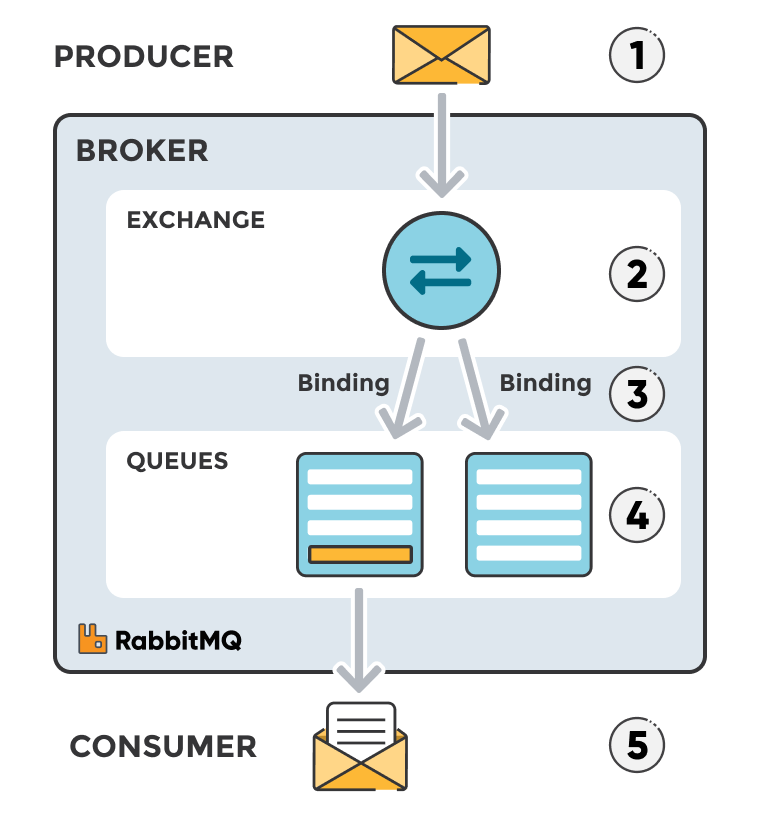
\includegraphics[width=0.5\textwidth]{styles/diploma/inc/rabbitmq2.png} 
    \caption{Устройство обменников в RabbitMQ}
    \label{fig:example}
\end{figure}







